\documentclass{article}
% General document formatting
\usepackage[margin=0.7in]{geometry}
\usepackage[parfill]{parskip}
\usepackage[utf8]{inputenc}
\usepackage{pdflscape}
\usepackage{tikz}

% Related to math
\usepackage{amsmath,amssymb,amsfonts,amsthm}

\usetikzlibrary{arrows.meta}
\usetikzlibrary{calc}

% notations
\newcommand{\Transform}[2]{^{#1}\textbf{T}_{#2}}
\newcommand{\Pose}[2]{^{#1}\textbf{P}_{#2}}
\newcommand{\Translation}[1]{\textbf{t}_{#1}}
\newcommand{\Rotation}[2]{^{#1}\textbf{R}_{#2}}
\newcommand{\Position}[2]{^{#1}\textbf{p}_{#2}}
\newcommand{\Yaw}[1]{^W\phi_{z_{#1}}}
% \newcommand{\Or}

% use custom tkiz drawings
%% -----------------------------------------------------------------------------------------------------------------
% Draws a wheel at given position and orientation.
% arguments:
% #1: position [x,y]
% #2: orientation [°]
\newcommand{\drawomiwheelleft}[2]{
    \begin{scope}[shift={(#1)}]
        \begin{scope}[rotate=#2]
            \draw [line width=0.4mm, draw=black] (-0.245,-0.42) rectangle ++(0.49,0.77);
            \draw [line width=0.2mm, fill=gray, rotate around={45:(0.21,0.07)}] (-0.345,-0.03) rectangle ++(0.42,0.14);
            \draw [line width=0.2mm, fill=gray, rotate around={45:(0.21,0.07)}] (-0.105, 0.21) rectangle ++(0.42,0.14);
        \end{scope}
    \end{scope}
}
\newcommand{\drawomiwheelright}[2]{
    \begin{scope}[shift={(#1)}]
        \begin{scope}[rotate=#2]
            \draw [line width=0.4mm, draw=black] (-0.245,-0.42) rectangle ++(0.49,0.77);
            % \draw [line width=0.2mm, draw=black, rotate around={-45:(0.21,0.07)}] ( 0.03,-0.32) rectangle ++(0.42,0.14);
            % \draw [line width=0.2mm, draw=black, rotate around={-45:(0.21,0.07)}] (-0.17,-0.09) rectangle ++(0.42,0.14);
            \draw [line width=0.2mm, fill=gray, rotate around={-45:(0.21,0.07)}] (0.03, -0.345) rectangle ++(0.42,0.14);
            \draw [line width=0.2mm, fill=gray, rotate around={-45:(0.21,0.07)}] (-0.21,-0.105) rectangle ++(0.42,0.14);
        \end{scope}
    \end{scope}
}
%% -----------------------------------------------------------------------------------------------------------------

%% -----------------------------------------------------------------------------------------------------------------
% Draws a coordinate system at given position and orientation. Additional a text label is printed as well without
% orientation. Note: position of text is buggy!
% #1: name [text]
% #2: position [x,y]
% #3: orientation [°]
\newcommand{\drawcoordinatesystem}[3]{
    \begin{scope}[shift={(#2)}]
        \begin{scope}[rotate=#3]
            \node (#1) at (0,0) {};
            \draw [-stealth, draw=red,   line width=0.5mm] (0,0) -- ( 0,1);
            \draw [-stealth, draw=green, line width=0.5mm] (0,0) -- (-1,0);
            \filldraw [fill=black] (0,0) circle (1mm);
        \end{scope}
        \node at (-0.5, -0.0) {#1};
    \end{scope}
}
%% -----------------------------------------------------------------------------------------------------------------

%% -----------------------------------------------------------------------------------------------------------------
% Draws a robot at given position and orientation. The given name will be printed at robot's origin.
% #1: name [text]
% #2: position [x,y]
% #3: orientation [°]
\newcommand{\drawrobot}[3]{
    \begin{scope}[shift={(#2)}]
        \begin{scope}[rotate=#3]
            \drawomiwheelright{0.84,-0.84}{0};
            \drawomiwheelleft{-0.84,-0.84}{0};
            \drawomiwheelleft{ 0.84, 0.84}{0};
            \drawomiwheelright{-0.84, 0.84}{0};
            \draw [draw=black, line width=0.4mm] (-0.5,-1.0) rectangle ++(1.0,2.0);
            \draw [draw=black, dashed, line width=0.3mm] (0,0) circle (1.1879);
        \end{scope}
    \end{scope}    
    \drawcoordinatesystem{#1}{#2}{#3}
}
%% -----------------------------------------------------------------------------------------------------------------


\begin{document}

\section{Kalman Filter Models for Mecanum Drive Kinematic}

This document defines the formulas required for a Kalman filter that is used to localize the EduArt robots globally.Several models are defined, each of which has its advantages and disadvantages. 

Basically, the movement in the model is linearized, even if an extended Kalman filter is used. This liberalizes around the current state. As a result, a circular path cannot be followed exactly. Instead, an under- or over-tracking occurs.

\begin{figure}
  \center
  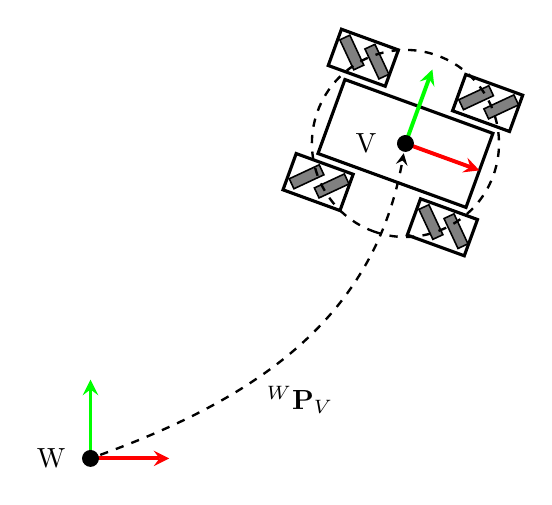
\begin{tikzpicture}
    \drawrobot{V}{4,4}{-110};
    \drawcoordinatesystem{W}{0,0}{-90};
    \draw [dashed, line width=0.3mm, -stealth] (W) to[out=20,in=-100] node[below, xshift=0cm, yshift=-4mm]{$\Pose{W}{V}$} (V);
    % \draw [dashed, line width=0.3mm, -stealth] (F$_j$) to[out=-90,in=-20] node[below, xshift=2mm, yshift=-2mm]{$\Transform{F_j}{R_{j,2}}$} (R$_{j,2}$);
    % \draw [dashed, line width=0.3mm, -stealth] (W) to[out= 20,in=-60] node[below, xshift=2mm, yshift=-2mm]{$\Transform{W}{F_j}$} (F$_j$);
    % \draw [dashed, line width=0.3mm, -stealth] (W) to[out= 50,in=-80] node[right, xshift=1mm, yshift= 0mm]{$\Transform{W}{R_{j,2}}$} (R$_{j,2}$);
\end{tikzpicture}

  \caption{General Overview}
  \label{fig:general_overview}
\end{figure}

\clearpage
\section{Model: Push and Rotate}

\begin{figure}
  \center

  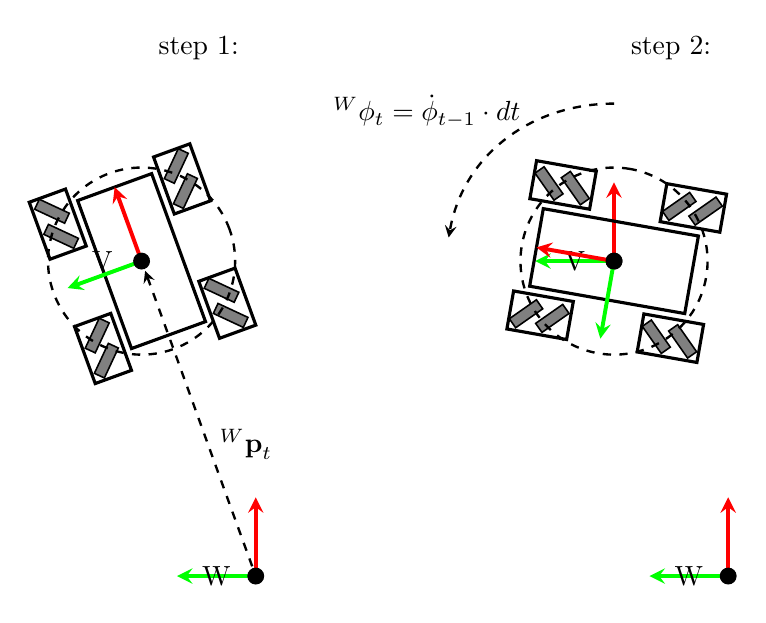
\begin{tikzpicture}
    % translation
    \node at (-0.725, 6.7) {step 1:};
    \drawcoordinatesystem{W}{0,0}{0};
    \drawrobot{V}{-1.45, 4}{20};
    \draw [dashed, line width=0.3mm, -stealth] (W) to[out=110,in=-70] node[below, xshift=6mm, yshift=0mm]{$\Position{W}{t}$} (V);
    % rotation
    \node at (5.275, 6.7) {step 2:};
    \draw [dashed, line width=0.3mm, -stealth] (4.55, 6) to[out=180,in=80] node[below, xshift=-10mm, yshift=7mm]{$^W\phi_t = \dot{\phi}_{t-1} \cdot dt$} (2.45, 4.3);
    \drawcoordinatesystem{W}{6, 0}{0};
    \drawcoordinatesystem{V}{4.55, 4}{0};
    \drawrobot{}{4.55, 4}{80};
  \end{tikzpicture}
  \caption{Push and Rotate}
  \label{fig:push_and_rotate}
\end{figure}


The model defined here first travels a distance based on the velocity and acceleration vectors. The robot is then rotated. We call this Push and Rotate.

\subsection{Prediction Model for Eduard with Mecanum}

\subsubsection{Acceleration}
\begin{align}
  \textbf{a}_{t-1} &= \left(\begin{matrix}a_{x_{t-1}}\\a_{y_{t-1}}\end{matrix}\right) \\
  \textbf{a}_t &= \textbf{a}_{t-1}
\end{align}

\subsubsection{Velocity}
\begin{align}
  \textbf{v}_{t-1} &= \left(\begin{matrix}v_{x_{t-1}}\\v_{y_{t-1}}\end{matrix}\right) \\
  \textbf{v}_t &= \textbf{v}_{t-1} + \textbf{a}_{t-1} dt = 
  \left(\begin{matrix}a_{x_{t-1}} dt + v_{x_{t-1}}\\a_{y_{t-1}} dt + v_{y_{t-1}}\end{matrix}\right)
\end{align}

\subsubsection{Yaw}
\begin{align}
  \Yaw{t} &= \Yaw{t-1} + \dot{\phi}_{z_{t-1}} dt \\
  \dot{\phi}_{z_t} &= \dot{\phi}_{z_{t-1}}
\end{align}

\subsubsection{Position}
\begin{align}
  \textrm{cos}_\phi &= \cos{\left(\Yaw{t-1}\right)} \\
  \textrm{sin}_\phi &= \sin{\left(\Yaw{t-1}\right)} \\
  \Rotation{W}{t-1} &= \left(\begin{matrix}\textrm{cos}_\phi & - \textrm{sin}_\phi\\\textrm{sin}_\phi & \textrm{cos}_\phi\end{matrix}\right) \\
  \Position{W}{t-1} &= \left(\begin{matrix}p_{x (t-1)}\\p_{y (t-1)}\end{matrix}\right) \\
  \Position{W}{t} &= \Position{W}{t-1} + \Rotation{W}{t-1}\textbf{v}_{t-1}dt + \frac{1}{2}\Rotation{W}{t-1}\textbf{a}_{t-1}dt^2 \\
  &= \left(\begin{matrix}dt^{2} \left(0.5 a_{x_{t-1}} \textrm{cos}_\phi - 0.5 a_{y_{t-1}} \textrm{sin}_\phi\right) + dt \left(v_{x_{t-1}} \textrm{cos}_\phi - v_{y_{t-1}} \textrm{sin}_\phi\right) + p_{x (t-1)}\\dt^{2} \left(0.5 a_{x_{t-1}} \textrm{sin}_\phi + 0.5 a_{y_{t-1}} \textrm{cos}_\phi\right) + dt \left(v_{x_{t-1}} \textrm{sin}_\phi + v_{y_{t-1}} \textrm{cos}_\phi\right) + p_{y (t-1)}\end{matrix}\right)
\end{align}

\subsubsection{Model}

\begin{align}
 \textbf{F}_{t} &=
 \left(\begin{matrix}
  p_{x_t} \\
  p_{y_t} \\
  v_{x_t} \\
  v_{y_t} \\
  a_{x_t} \\
  a_{y_t} \\
  \phi_t \\
  \dot{\phi_t}
 \end{matrix}\right)
 = \left(\begin{matrix}dt^{2} \left(0.5 a_{x_{t-1}} \textrm{cos}_\phi - 0.5 a_{y_{t-1}} \textrm{sin}_\phi\right) + dt \left(v_{x_{t-1}} \textrm{cos}_\phi - v_{y_{t-1}} \textrm{sin}_\phi\right) + p_{x (t-1)}\\dt^{2} \left(0.5 a_{x_{t-1}} \textrm{sin}_\phi + 0.5 a_{y_{t-1}} \textrm{cos}_\phi\right) + dt \left(v_{x_{t-1}} \textrm{sin}_\phi + v_{y_{t-1}} \textrm{cos}_\phi\right) + p_{y (t-1)}\\a_{x_{t-1}} dt + v_{x_{t-1}}\\a_{y_{t-1}} dt + v_{y_{t-1}}\\a_{x_{t-1}}\\a_{y_{t-1}}\\\dot{\phi}_{z_{t-1}} dt + \phi_{z_{t-1}}\\\dot{\phi}_{z_{t-1}}\end{matrix}\right) \\
  \textbf{J}_t &= 
  \textbf{F}\left(\begin{matrix}
    \frac{\partial}{\partial p_x} & \frac{\partial}{\partial p_y} & \frac{\partial}{\partial v_x} & \frac{\partial}{\partial v_y} & \frac{\partial}{\partial a_x} & \frac{\partial}{\partial a_y} & 0 & \frac{\partial}{\partial \dot{\phi}}
  \end{matrix}\right) \\
  &= \left(\begin{matrix}1 & 0 & dt \textrm{cos}_\phi & - dt \textrm{sin}_\phi & 0.5 dt^{2} \textrm{cos}_\phi & - 0.5 dt^{2} \textrm{sin}_\phi & 0 & 0\\0 & 1 & dt \textrm{sin}_\phi & dt \textrm{cos}_\phi & 0.5 dt^{2} \textrm{sin}_\phi & 0.5 dt^{2} \textrm{cos}_\phi & 0 & 0\\0 & 0 & 1 & 0 & dt & 0 & 0 & 0\\0 & 0 & 0 & 1 & 0 & dt & 0 & 0\\0 & 0 & 0 & 0 & 1 & 0 & 0 & 0\\0 & 0 & 0 & 0 & 0 & 1 & 0 & 0\\0 & 0 & 0 & 0 & 0 & 0 & 1 & dt\\0 & 0 & 0 & 0 & 0 & 0 & 0 & 1\end{matrix}\right)
\end{align}

\section{System Noise Model}
\subsubsection{Via Acceleration}

The system noise is partly determined by the acceleration that the robot can experience.

\begin{align}
  a &= a_x = a_y \\
  \textbf{a} &= \left(\begin{matrix}a\\a\end{matrix}\right) \\
  \textbf{v} &= \left(\begin{matrix}a \cdot dt\\a \cdot dt\end{matrix}\right) \\
  \textbf{p} &= \frac{1}{2}\textbf{R}_{t-1}\textbf{a} \cdot dt^2 \\ 
  &= \left(\begin{matrix}dt^{2} \left(- 0.5 \cdot a \cdot \textrm{sin}_\phi + 0.5 \cdot a \cdot \textrm{cos}_\phi\right)\\dt^{2} \left(0.5 \cdot a \cdot \textrm{sin}_\phi + 0.5 \cdot a \cdot \textrm{cos}_\phi\right)\end{matrix}\right) \\
  \textbf{a}_{\textrm{noise}} =
  \left(\begin{matrix}
    \textbf{p} \\
    \textbf{v} \\
    \textbf{a} \\
    0 \\
    0
  \end{matrix}\right)
&=\left(\begin{matrix}0.5 \sqrt{2} dt^{2} \cos{\left(\phi_{z_{t-1}} + \frac{\pi}{4} \right)}\\0.5 \sqrt{2} dt^{2} \sin{\left(\phi_{z_{t-1}} + \frac{\pi}{4} \right)}\\dt\\dt\\1\\1\\0\\0\end{matrix}\right) a
\end{align}

\begin{equation}
  \textbf{Q}_{\textbf{a}} = \sigma^2_{\textbf{a}} \cdot \textbf{a}_{\textrm{noise}} \cdot \textbf{a}_{\textrm{noise}}^T \\
  = \sigma^2_{\textbf{a}} \left(\begin{matrix}\frac{p_{x}^{2}}{a^{2}} & \frac{p_{x} p_{y}}{a^{2}} & \frac{dt p_{x}}{a} & \frac{dt p_{x}}{a} & \frac{p_{x}}{a} & \frac{p_{x}}{a} & 0 & 0\\\frac{p_{x} p_{y}}{a^{2}} & \frac{p_{y}^{2}}{a^{2}} & \frac{dt p_{y}}{a} & \frac{dt p_{y}}{a} & \frac{p_{y}}{a} & \frac{p_{y}}{a} & 0 & 0\\\frac{dt p_{x}}{a} & \frac{dt p_{y}}{a} & dt^{2} & dt^{2} & dt & dt & 0 & 0\\\frac{dt p_{x}}{a} & \frac{dt p_{y}}{a} & dt^{2} & dt^{2} & dt & dt & 0 & 0\\\frac{p_{x}}{a} & \frac{p_{y}}{a} & dt & dt & 1 & 1 & 0 & 0\\\frac{p_{x}}{a} & \frac{p_{y}}{a} & dt & dt & 1 & 1 & 0 & 0\\0 & 0 & 0 & 0 & 0 & 0 & 0 & 0\\0 & 0 & 0 & 0 & 0 & 0 & 0 & 0\end{matrix}\right)
\end{equation}


\subsubsection{Via Yaw Rate}

The system noise is partly determined by the yaw rate that the robot can experience.

\begin{align}
  \phi_z &= \dot{\phi_{z}} dt \\
  \dot{\phi}_{z_\textrm{noise}} &= \left(\begin{matrix}0\\0\\0\\0\\0\\0\\\phi_z\\\dot{\phi_z}\end{matrix}\right) =
  \left(\begin{matrix}0\\0\\0\\0\\0\\0\\dt\\1\end{matrix}\right) \dot{\phi_z}
\end{align}

\begin{align}
  \textbf{Q}_{\textrm{yaw}} &= \sigma^2_{\textrm{yaw}} \cdot \dot{\phi}_{z_\textrm{noise}} \cdot \dot{\phi}_{z_\textrm{noise}}^T
  = \sigma^2_{\textrm{yaw}} \left(\begin{matrix}0 & 0 & 0 & 0 & 0 & 0 & 0 & 0\\0 & 0 & 0 & 0 & 0 & 0 & 0 & 0\\0 & 0 & 0 & 0 & 0 & 0 & 0 & 0\\0 & 0 & 0 & 0 & 0 & 0 & 0 & 0\\0 & 0 & 0 & 0 & 0 & 0 & 0 & 0\\0 & 0 & 0 & 0 & 0 & 0 & 0 & 0\\0 & 0 & 0 & 0 & 0 & 0 & dt^{2} & dt\\0 & 0 & 0 & 0 & 0 & 0 & dt & 1\end{matrix}\right)
\end{align}

\subsubsection{Final System Noise Matrix}

\begin{align}
  \textbf{Q} &= \textbf{Q}_{\textbf{j}} + \textbf{Q}_{\textrm{yaw}}
  = \left(\begin{matrix}\frac{\sigma^2_\textbf{a} p_{x}^{2}}{a^{2}} & \frac{\sigma^2_\textbf{a} p_{x} p_{y}}{a^{2}} & \frac{\sigma^2_\textbf{a} dt p_{x}}{a} & \frac{\sigma^2_\textbf{a} dt p_{x}}{a} & \frac{\sigma^2_\textbf{a} p_{x}}{a} & \frac{\sigma^2_\textbf{a} p_{x}}{a} & 0 & 0\\\frac{\sigma^2_\textbf{a} p_{x} p_{y}}{a^{2}} & \frac{\sigma^2_\textbf{a} p_{y}^{2}}{a^{2}} & \frac{\sigma^2_\textbf{a} dt p_{y}}{a} & \frac{\sigma^2_\textbf{a} dt p_{y}}{a} & \frac{\sigma^2_\textbf{a} p_{y}}{a} & \frac{\sigma^2_\textbf{a} p_{y}}{a} & 0 & 0\\\frac{\sigma^2_\textbf{a} dt p_{x}}{a} & \frac{\sigma^2_\textbf{a} dt p_{y}}{a} & \sigma^2_\textbf{a} dt^{2} & \sigma^2_\textbf{a} dt^{2} & \sigma^2_\textbf{a} dt & \sigma^2_\textbf{a} dt & 0 & 0\\\frac{\sigma^2_\textbf{a} dt p_{x}}{a} & \frac{\sigma^2_\textbf{a} dt p_{y}}{a} & \sigma^2_\textbf{a} dt^{2} & \sigma^2_\textbf{a} dt^{2} & \sigma^2_\textbf{a} dt & \sigma^2_\textbf{a} dt & 0 & 0\\\frac{\sigma^2_\textbf{a} p_{x}}{a} & \frac{\sigma^2_\textbf{a} p_{y}}{a} & \sigma^2_\textbf{a} dt & \sigma^2_\textbf{a} dt & \sigma^2_\textbf{a} & \sigma^2_\textbf{a} & 0 & 0\\\frac{\sigma^2_\textbf{a} p_{x}}{a} & \frac{\sigma^2_\textbf{a} p_{y}}{a} & \sigma^2_\textbf{a} dt & \sigma^2_\textbf{a} dt & \sigma^2_\textbf{a} & \sigma^2_\textbf{a} & 0 & 0\\0 & 0 & 0 & 0 & 0 & 0 & \sigma_{\dot{\phi_z}}^2 dt^{2} & \sigma_{\dot{\phi_z}}^2 dt\\0 & 0 & 0 & 0 & 0 & 0 & \sigma_{\dot{\phi_z}}^2 dt & \sigma_{\dot{\phi_z}}^2\end{matrix}\right)
\end{align}
\clearpage



\section{Model: Rotate and Push}

\begin{figure}
  \center

  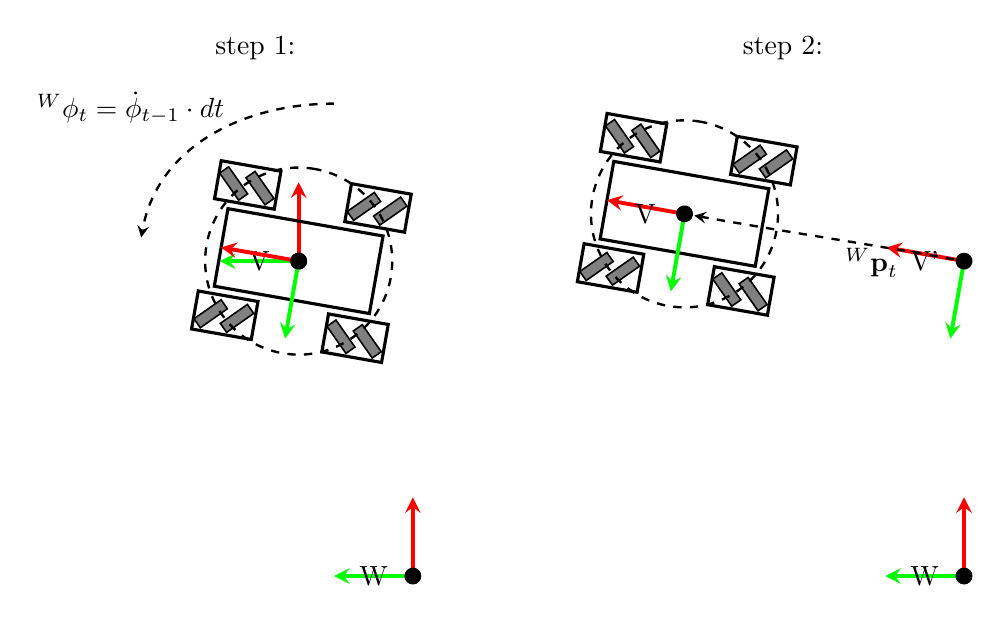
\begin{tikzpicture}
    % rotation
    \node at (-2, 6.7) {step 1:};
    \draw [dashed, line width=0.3mm, -stealth] (-1, 6) to[out=180,in=80] node[below, xshift=-10mm, yshift=7mm]{$^W\phi_t = \dot{\phi}_{t-1} \cdot dt$} (-3.45, 4.3);
    \drawcoordinatesystem{W}{0, 0}{0};
    \drawcoordinatesystem{V}{-1.45, 4}{0};
    \drawrobot{}{-1.45, 4}{80};
    % translation
    \node at (4.7, 6.7) {step 2:};
    \drawcoordinatesystem{W}{7, 0}{0};
    \drawcoordinatesystem{V'}{7, 4}{80}
    \drawrobot{V}{3.45, 4.6}{80};
    \draw [dashed, line width=0.3mm, -stealth] (V') to[out=170,in=-10] node[below, xshift=6mm, yshift=0mm]{$\Position{W}{t}$} (V);
  \end{tikzpicture}
  \caption{Push and Rotate}
  \label{fig:push_and_rotate}
\end{figure}



\end{document}